\documentclass[a4paper,11.5pt]{article} % тип документа


%%%Библиотеки
%\usepackage[warn]{mathtext}	
%\usepackage[T2A]{fontenc} % кодировка
\usepackage[utf8]{inputenc} % кодировка исходного текста
\usepackage[english,russian]{babel} % локализация и переносы
\usepackage{caption}
\usepackage{listings}
\usepackage{amsmath,amsfonts,amssymb,amsthm,mathtools}
\usepackage{wasysym}
\usepackage{graphicx}%Вставка картинок правильная
\usepackage{float}%"Плавающие" картинки
\usepackage{wrapfig}%Обтекание фигур (таблиц, картинок и прочего)
\usepackage{fancyhdr} %загрузим пакет
\usepackage{lscape}
\usepackage{xcolor}
\usepackage[normalem]{ulem}
\usepackage{hyperref}

\usepackage{mathtext}
\newcommand{\angstrom}{\text{\normalfont\AA}}
%%%Конец библиотек


%%%Настройка ссылок
\hypersetup
{
	colorlinks=true,
	linkcolor=blue,
	filecolor=magenta,
	urlcolor=blue
}
%%%Конец настройки ссылок


%%%Настройка колонтитулы
\pagestyle{fancy}
\fancyhead{}
\fancyhead[L]{Лабораторная работа 1}
\fancyhead[R]{Курневич Станислав, группа Б01-008а}
\fancyfoot[C]{\thepage}
%%%конец настройки колонтитулы



\begin{document}
	%%%%Начало документа%%%%
	
	%%%Начало титульника
	
	\begin{titlepage}
		
		\newpage
		\begin{center}
			\normalsize Московский физико-технический институт \\(госудраственный 			университет)
		\end{center}
		
		\vspace{6em}
		
		\begin{center}
			\Large Лабораторная работа по вычислительно математике\\
		\end{center}
		
		\vspace{1em}
		
		\begin{center}
			\large \textbf{Лабораторная работа 1}
		\end{center}
		
		\vspace{2em}
		
		\begin{center}
			\large Работу выполнил:\\	
			Курневич Станислав Витальевич\\
			Группа Б01-008а
		\end{center}
		
		\vspace{\fill}
		
		\begin{center}
			Долгопрудный \\27.09.2022
		\end{center}
		
	\end{titlepage}
	%%%Конец Титульника
	
	%%%%%%Начало работы с текстом%%%%%%
	
    \section{Постановка задачи}
    
    Построить графики абсолютной погрешности каждого метода численного вычисления производной в зависимости от шага численного дифференцирования $h_n = \frac{2}{2^n},~ n = \overline{1, 21}$ для функций
    \begin{enumerate}
        \item $\sin(x^2)$
        \item $\cos(\sin(x))$
        \item $\exp(\sin(\cos(x)))$
        \item $ln(x + 3)$
        \item $(x + 3)^{0.5}$
    \end{enumerate}

    \section{Построение графиков}
    Для каждой функции используется 5 методов приближенного вычисления производной:
    \begin{enumerate}
        \item $\frac{f(x + h) - f(x)}{h}$
        \item $\frac{f(x) - f(x - h)}{h}$
        \item $\frac{f(x + h) - f(x - h)}{2h}$
        \item $\frac{4}{3}\frac{f(x + h) - f(x - h)}{2h} - \frac{1}{3}\frac{f(x + 2h) - f(x - 2h)}{4h}$
        \item $\frac{3}{2}\frac{f(x + h) - f(x - h)}{2h} - \frac{3}{5}\frac{f(x + 2h) - f(x - 2h)}{4h} + \frac{1}{10}\frac{f(x + 3h) - f(x - 3h)}{6h}$
    \end{enumerate}

    Графики строятся в логарифмическом маштабе по обеим осям.

    \begin{figure}[H]
		\center{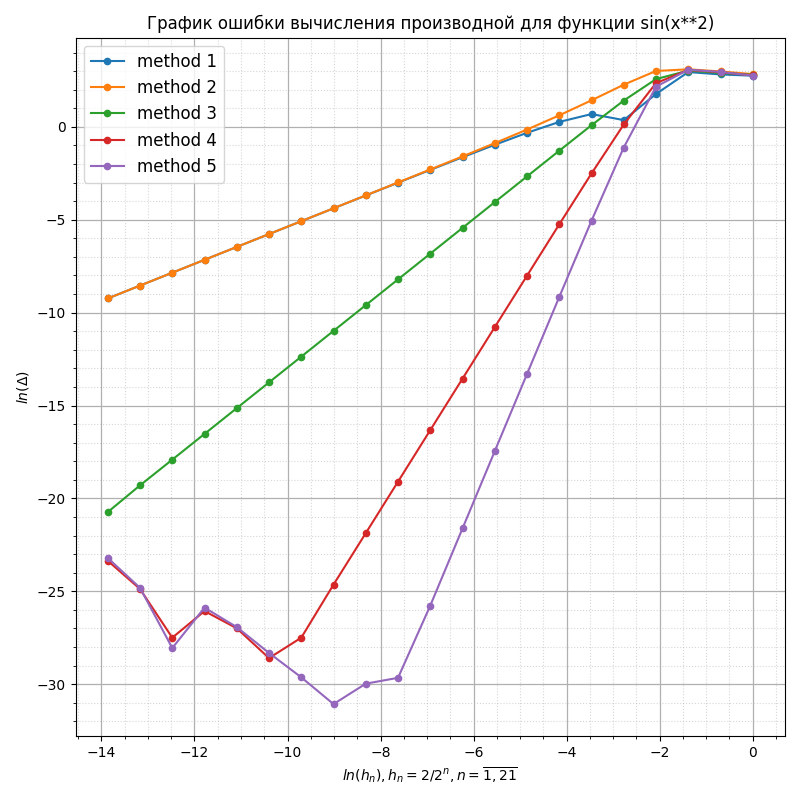
\includegraphics[scale = 0.4]{images/fsin(x**2).png}}
	\end{figure}

    \begin{figure}[H]
		\center{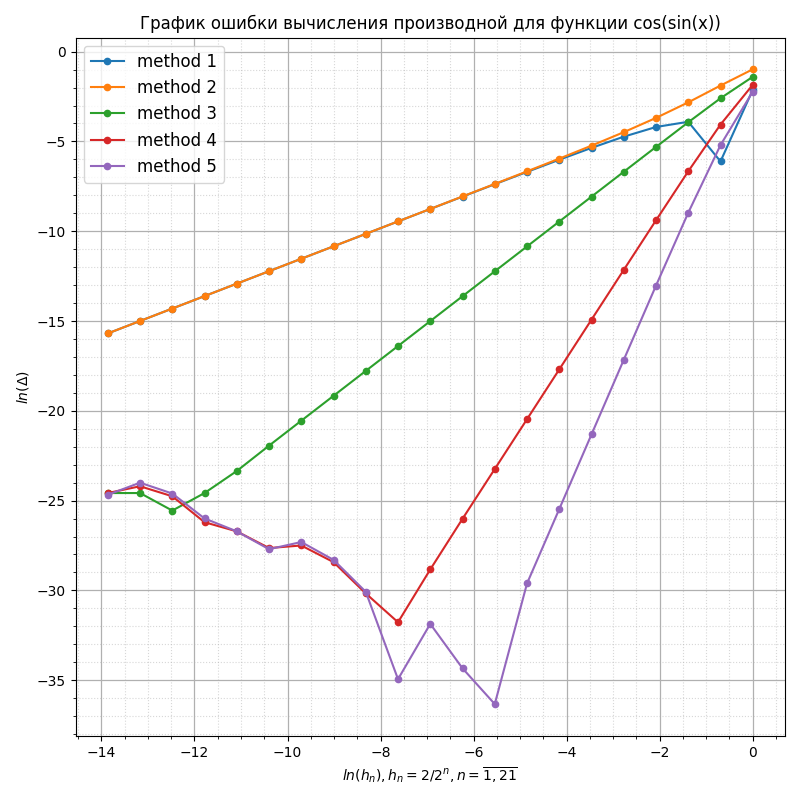
\includegraphics[scale = 0.4]{images/fcos(sin(x)).png}}
	\end{figure}

    \begin{figure}[H]
		\center{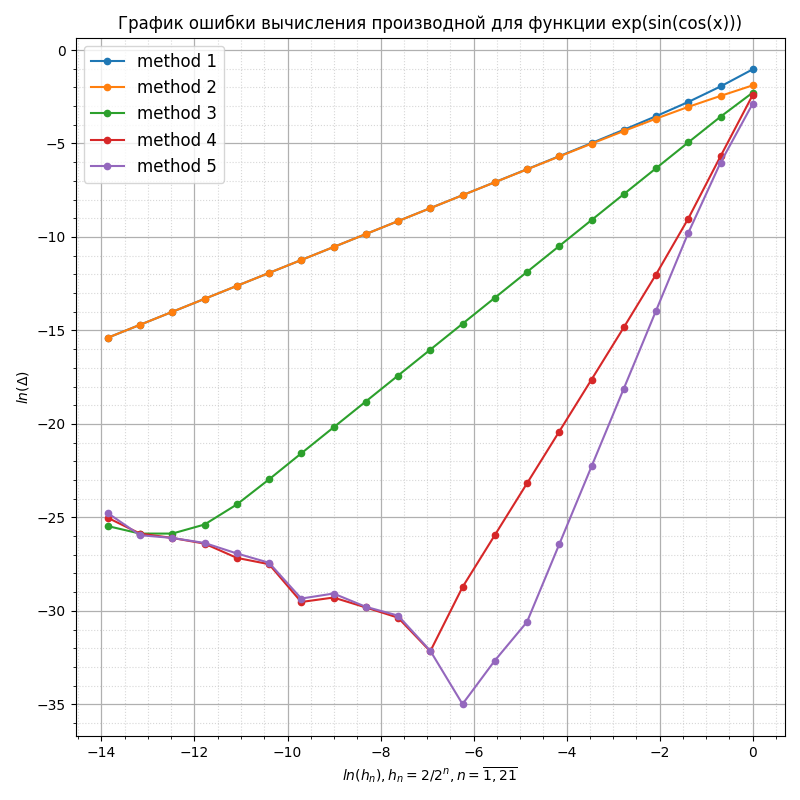
\includegraphics[scale = 0.4]{images/fexp(sin(cos(x))).png}}
	\end{figure}

    \begin{figure}[H]
		\center{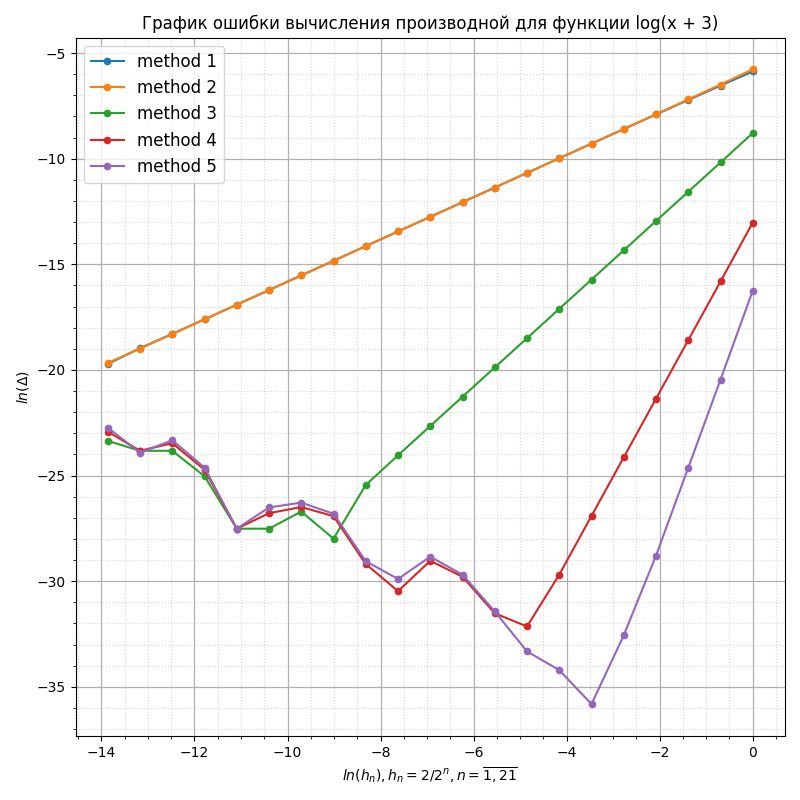
\includegraphics[scale = 0.4]{images/flog(x + 3).png}}
	\end{figure}

    \begin{figure}[H]
		\center{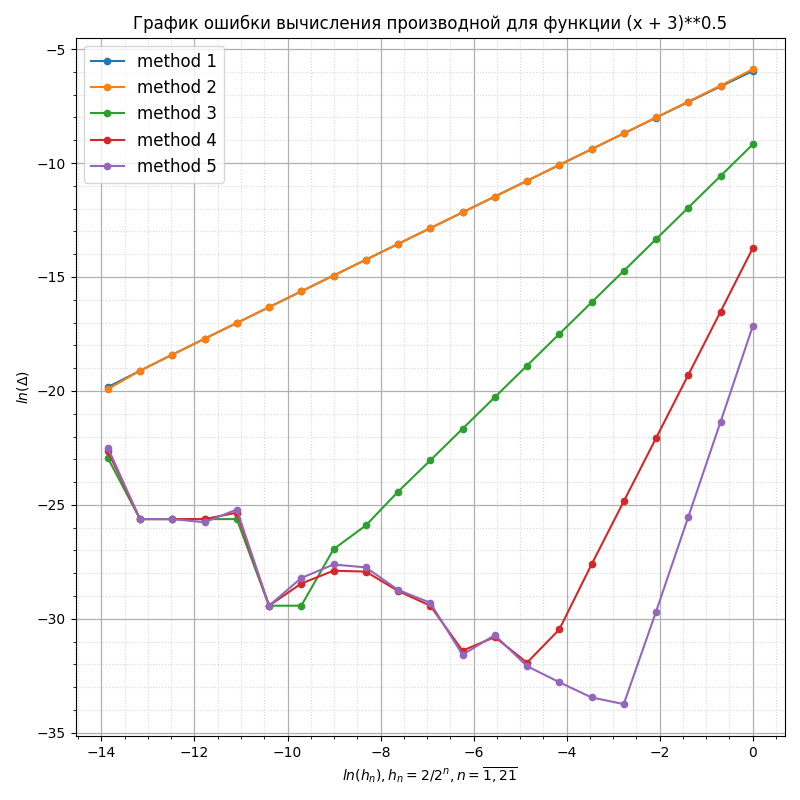
\includegraphics[scale = 0.4]{images/f(x + 3)**0.5.png}}
	\end{figure}

\end{document}